%% REPLACE sXXXXXXX with your student number
\def\studentNumber{S25697578}


%% START of YOUR ANSWERS
%% Add answers to the questions below, by replacing the text inside the brackets {} for \youranswer{ "Text to be replaced with your answer." }. 
%
% Do not delete the commands for adding figures and tables. Instead fill in the missing values with your experiment results, and replace the images with your own respective figures.
%
% You can generally delete the placeholder text, such as for example the text "Question Figure 3 - Replace the images ..." 
%
% There are 5 TEXT QUESTIONS. Replace the text inside the brackets of the command \youranswer with your answer to the question.
%
% There are also 3 "questions" to replace some placeholder FIGURES with your own, and 1 "question" asking you to fill in the missing entries in the TABLE provided. 
%
% NOTE! that questions are ordered by the order of appearance of their answers in the text, and not necessarily by the order you should tackle them. You should attempt to fill in the TABLE and FIGURES before discussing the results presented there. 
%
% NOTE! If for some reason you do not manage to produce results for some FIGURES and the TABLE, then you can get partial marks by discussing your expectations of the results in the relevant TEXT QUESTIONS. The TABLE specifically has enough information in it already for you to draw meaningful conclusions.
%
% Please refer to the coursework specification for more details.


%% - - - - - - - - - - - - TEXT QUESTIONS - - - - - - - - - - - - 

%% Question 1:
\newcommand{\questionOne} {
\youranswer{From Figure 2 and 3, we can see that there is a healthy amount of gradient flow across the different layers of VGG 08 model, but not the VGG 38 model. This indicates that the gradient is not flowing properly through the layers of the VGG 38 model pointing that it suffers from a vanishing gradient problem which is hampering the training of the model. 
This is further supported by Figure 1 (a) and (b) which show that the loss of the VGG 38 model remains high while the accuracy being very low on both the training and the validation datasets.}
}
% Question 1 - Use Figures 1, 2, and 3 to identify the Vanishing Gradient Problem (which of these model suffers from it, and what are the consequences depicted?).
% The average length for an answer to this question is approximately 1/5 of the columns in a 2-column page

%% Question 2:
\newcommand{\questionTwo} {
\youranswer{Question 2 - Consider these results (including Figure 1 from \cite{he2016deep}). Discuss the relation between network capacity and overfitting, and whether, and how, this is reflected on these results. What other factors may have lead to this difference in performance?

The average length for an answer to this question is
approximately 1/5 of the columns in a 2-column page}
}

%% Question 3:
\newcommand{\questionThree} {
\youranswer{Question 3 - In this coursework, we didn't incorporate residual connections to the downsampling layers. Explain and justify what would need to be changed in order to add residual connections to the downsampling layers. Give and explain 2 ways of incorporating these changes and discuss pros and cons of each.
}
}

%% Question 4:
\newcommand{\questionFour} {
\youranswer{Question 4 - Present and discuss the experiment results (all of the results and not just the ones you had to fill in) in Table 1 and Figures 4 and 5 (you may use any of the other Figures if you think they are relevant to your analysis). You will have to determine what data are relevant to the discussion, and what information can be extracted from it. Also, discuss what further experiments you would have ran on any combination of VGG08, VGG38, BN, RC in order to
\begin{itemize}
    \item Improve performance of the model trained (explain why you expect your suggested experiments will help with this).
    \item Learn more about the behaviour of BN and RC (explain what you are trying to learn and how).
\end{itemize}

The average length for an answer to this question is approximately 1 of the columns in a 2-column page
}
}


%% Question 5:
\newcommand{\questionFive} {
\youranswer{Question 5 - Briefly draw your conclusions based on the results from the previous sections (what are the take-away messages?) and conclude your report with a recommendation for future work. 

Good recommendations for future work also draw on the broader literature (the papers already referenced are good starting points). Great recommendations for future work are not just incremental (an example of an incremental suggestion would be: ``we could also train with different learning rates'') but instead also identify meaningful questions or, in other words, questions with answers that might be somewhat more generally applicable. 

For example, \citep{huang2017densely} end with \begin{quote}``Because of their compact internal representations and reduced feature redundancy, DenseNets may be good feature extractors for various computer vision tasks that build on convolutional features, e.g.,  [4,5].''\end{quote} 

while \cite{bengio1993problem} state in their conclusions that \begin{quote}``There remains theoretical questions to be considered,  such as whether the problem with simple gradient descent  discussed in this paper would be observed with  chaotic attractors that are not  hyperbolic.''\\\end{quote}

The length of this question description is indicative of the average length of a conclusion section}
}


%% - - - - - - - - - - - - FIGURES - - - - - - - - - - - - 

%% Question Figure 3:
\newcommand{\questionFigureThree} {
\youranswer{Question Figure 3 - Replace this image with a figure depicting the average gradient across layers, for the VGG38 model.

\textit{(The provided figure is correct, and can be used in your analysis. It is partially obscured so you can get credit for producing your own copy).}
%
\begin{figure}[t]
    \centering
    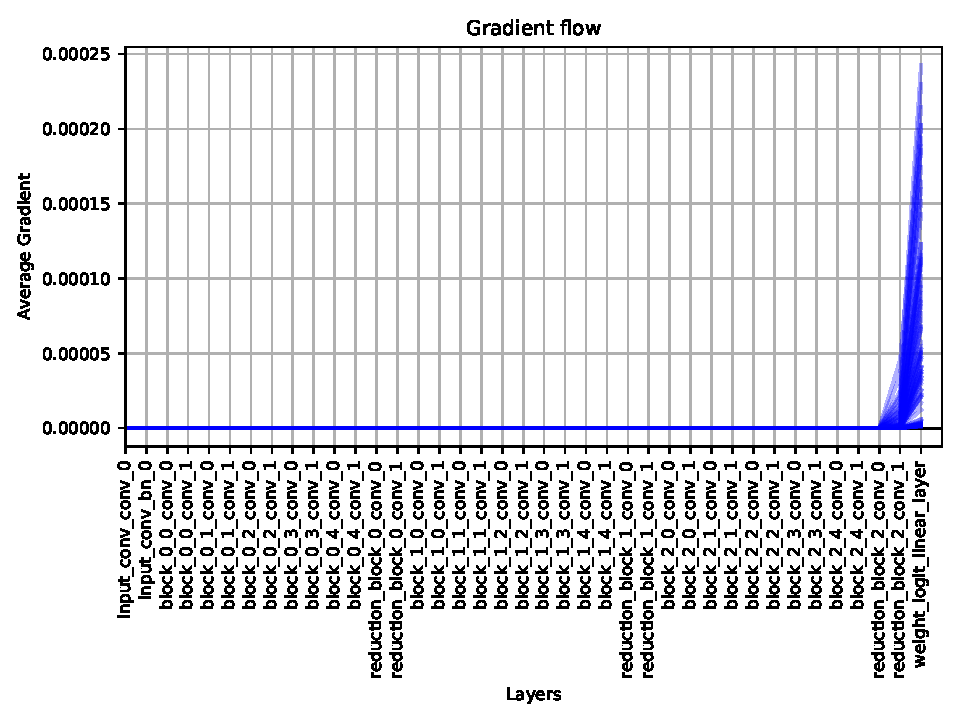
\includegraphics[width=\linewidth]{figures/gradplot_38.pdf}
    \caption{Gradient Flow on VGG38}
    \label{fig:grad_flow_38}
\end{figure}
}
}

%% Question Figure 4:
\newcommand{\questionFigureFour} {
\youranswer{Question Figure 4 - Replace this image with a figure depicting the training curves for the model with the best performance \textit{across experiments you have available (you don't need to run the experiments for the models we already give you results for)}. Edit the caption so that it clearly identifies the model and what is depicted.
%
\begin{figure}[t]
    \centering
    \includegraphics[width=\linewidth]{example-image-duck}
    \caption{Training curves for ? ? ?}
    \label{fig:grad_flow_bestModel}
\end{figure}
}
}

%% Question Figure 5:
\newcommand{\questionFigureFive} {
\youranswer{Question Figure 5 - Replace this image with a figure depicting the average gradient across layers, for the model with the best performance \textit{across experiments you have available (you don't need to run the experiments for the models we already give you results for)}. Edit the caption so that it clearly identifies the model and what is depicted.
%
\begin{figure}[t]
    \centering
    \includegraphics[width=\linewidth]{example-image-duck}
    \caption{Gradient Flow on ? ? ?}
    \label{fig:grad_flow_bestModel}
\end{figure}
}
}

%% - - - - - - - - - - - - TABLES - - - - - - - - - - - - 

%% Question Table 1:
\newcommand{\questionTableOne} {
\youranswer{
Question Table 1 - Fill in Table 1 with the results from your experiments on 
\begin{enumerate}
    \item \textit{VGG38 BN (LR 1e-3)}, and 
    \item \textit{VGG38 BN + RC (LR 1e-2)}.
\end{enumerate}
%
\begin{table*}[t]
    \centering
    \begin{tabular}{lr|ccccc}
    \toprule
        Model                   & LR   & \# Params & Train loss & Train acc & Val loss & Val acc \\
    \midrule
        VGG08                   & 1e-3 & 60 K      &  1.74      & 51.59     & 1.95     & 46.84 \\
        VGG38                   & 1e-3 & 336 K     &  4.61      & 00.01     & 4.61     & 00.01 \\
        VGG38 BN                & 1e-3 &     ?     &     ?      &     ?     &    ?     &     ? \\
        VGG38 RC                & 1e-3 & 336 K     &  1.33      & 61.52     & 1.84     & 52.32 \\
        VGG38 BN + RC           & 1e-3 & 339 K     &  1.26      & 62.99     & 1.73     & 53.76 \\
        VGG38 BN                & 1e-2 & 339 K     &  1.70      & 52.28     & 1.99     & 46.72 \\
        VGG38 BN + RC           & 1e-2 &     ?     &     ?      &     ?     &    ?     &     ? \\
    \bottomrule
    \end{tabular}
    \caption{Experiment results (number of model parameters, Training and Validation loss and accuracy) for different combinations of VGG08, VGG38, Batch Normalisation (BN), and Residual Connections (RC), LR is learning rate.}
    \label{tab:CIFAR_results}
\end{table*} 
}
}

%% END of YOUR ANSWERS
